\chapter{Ausblicke: C++}
\epigraph{C makes it easy to shoot yourself in the foot; C++ makes it harder, but when you do it blows your whole leg off.}{Bjarne Stroustrup}

\begin{plusbox}[keine grafische Hervorhebung von C++-Themen in diesem Kapitel]
Wie der Titel verspricht, behandelt dieses gesamte Kapitel Inhalte zur Sprache C++. Auf eine grafische Hervorhebung wird hier daher verzichtet.
\end{plusbox}

Einer der größten Vorteile der Sprache C ist seine Nähe zur Hardware, die es erlaubt, extrem effiziente Programme zu erstellen. Einer der größte Nachteile der Sprache C ist ebenfalls diese Hardware-Nähe, zwingt sie doch dazu, in abstrakten und kleinschrittigen Konzepten zu denken.

Die Sprache C++ wurde geschaffen, um die Effizienz von C so weit wie möglich zu erhalten, dabei aber menschennähere Denkweise in das Programmieren einzführen. Vielfach wiederkehrende Aufgaben sind in der STL (C++ Standard Library) in allgemeiner Form gelöst und können ohne weiteren Aufwand in eigene Projekte eingefügt werden\footnote{Der Name C++ leitet sich vom Inkrement-Operator \texttt{++} der Sprache C ab: C++ ist eine \emph{Aufwertung} der Sprache C. Einem ähnlichen Schema folgt auch die Benennung der Sprache C\# (sprich: C-sharp). Diese Weiterentwicklung von C++ sollte ursprünglich mit vier Pluszeichen geschrieben werden, eben als \emph{Aufwertung} von C++. Da dies aber in der Praxis zu umständlich wäre, ordnete man die Pluszeichen so um, dass sie das Raute-Symbol \# ergeben.}.

Syntaktisch sind sich C und C++ sehr ähnlich. Je nach gewähltem Compiler lässt sich C-Code mit einem C++-Compiler direkt umsetzen oder bedarf nur kleinerer Änderungen, um ein \emph{funktionierendes} Programm zu erzeugen. Dies soll aber nicht den Eindruck erwecken, C++ sei nur eine Variation der Sprache C. Vielmehr handelt es sich um eine komplette Neuentwicklung. Während C-Code von einem C++-Compiler zu einem \emph{funktionierenden} ausführbaren Programm umgesetzt werden kann, sieht \emph{guter} C++-Code bedeutend anders aus.

\begin{warnbox}[C++ ist eine eigenständige Sprache]
Einsteiger kommen ob der syntaktischen Nähe oft zu dem Schluss, dass C und C++ quasi dieselbe Sprache seien. Infolge dessen werden Code-Konzepte gemischt, was im besten Fall nur zu Performance-Einbußen oder eingeschränkter Kompatiblität des Codes mit verschiedenen Plattformen führt, im schlimmsten Fall aber zu instabilem Code und schwer auffindbaren Fehlern. Wenn Sie die Sprache C++ erlernen wollen -- wozu ich ihnen stark rate -- behalten Sie immer im Kopf, dass es sich um eine eigenständige Sprache handelt. Benutzen Sie Nachschlagewerke oder fragen Sie Dozenten und erfahrene ProgrammiererInnen in Ihrem Bekanntenkreis, ob sich eine Ihnen aus C bekannte Technik problemlos nach C++ übersetzen lässt.
\end{warnbox}

Aus Gründen des Umfangs kann hier nur ein \enquote{Teaser} für die Features der Sprache C++ gegeben werden. Eine tiefere Einsicht bietet der Kurs \emph{C++ und Qt} der Universität Regensburg. Für das Selbststudium ist das Tutorial (in englischer Sprache) unter \url{http://www.cplusplus.com/doc/tutorial/} sehr gut geeignet. Selbstverständlich ersetzt dieser Kurz-Kurs nicht die Praxis-Erfahrung (vgl. Abbildung \ref{fig:gooseCPP}), die Sie sich hoffentlich bald aneignen -- sowohl in C wie auch in C++.

\begin{figure}
	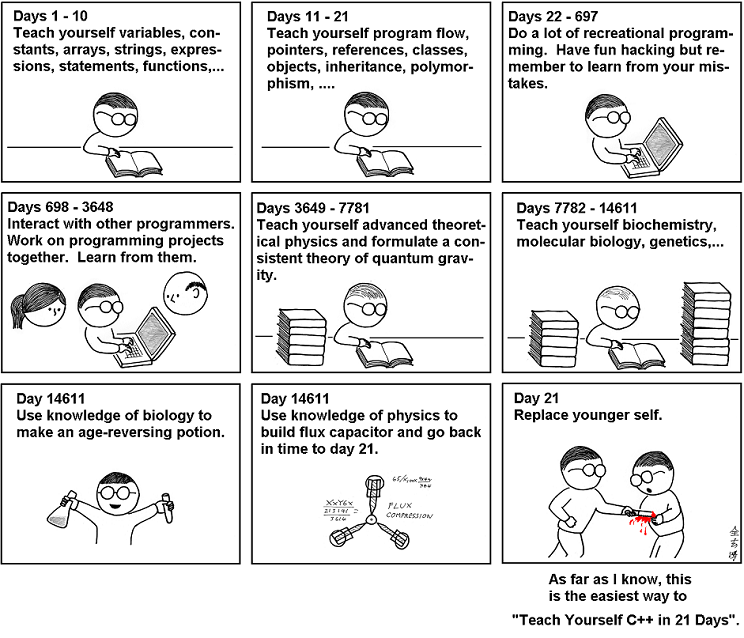
\includegraphics[width=\linewidth]{./gfx/agoose-249}
	\caption
		[Teach Yourself C++ in 21 days -- ein Praxisbericht.]
		{Teach Yourself C++ in 21 days -- ein Praxisbericht.\newline 
		 Quelle: \url{https://abstrusegoose.com/249}}
	\label{fig:gooseCPP}
\end{figure}


\section{Default Arguments und Function Overloading}
In C++ ist es möglich, Funktionen, die Parameter erwarten, Standardwerte vorzugeben. Beim Aufruf kann man dann diesen Parameter auslassen. Im Prototypen der Funktion wird dazu einfach hinter der Deklaration des Parameters ein \texttt{= Wert} angefügt. In der Kopfzeile der eigentlichen Funktion wird dies dann nicht mehr wiederholt.

\begin{codebox}[Beispiel: Funktion mit Default-Parameter]
\begin{minted}[linenos]{c++}
#include <iostream>

void showANumber(int number = 42);

void showANumber(int number) {
  std::cout << number << std::endl;
}

int main() {
   showANumber();
   showANumber(666);
}
\end{minted}
\end{codebox}

\begin{cmdbox}[Ausgabebeispiel: Funktion mit Default-Parameter]
42\\
666
\end{cmdbox}

\emph{Fakultative} (notwendige) und optionale Parameter (also solche, für die ein Standardwert vorgegeben wurde) können gemischt vorkommen; die optionalen Parameter müssen allerdings am Ende der Deklaration stehen.

Daneben ist es möglich, mehrere Funktionen mit demselben Bezeichner anzulegen, solange sich diese in der Signatur unterscheiden. Beispielsweise kann sich der Rückgabetyp unterscheiden oder die Zahl und Art der Parameter verschieden sein. Wir nennen dies \emph{Function Overloading}

Im Folgenden Beispiel benutzen wir Function Overloading, um mit einem Symbol Matrizen verschiedenen Datentyps (\mintinline{c++}{float} oder \mintinline{c++}{double}) anzulegen. Die Befehle \mintinline{c++}{new} und \mintinline{c++}{delete} sind für Sie noch neu, entsprechen in ihrer Funktion aber den Ihnen schon bekannten Befehlen \texttt{malloc} und \texttt{free}:

\begin{codebox}[Beispiel: Überladene Funktion]
\begin{minted}[linenos]{c++}
typedef struct {
  int     rows;
  int     cols;
  float*  data;
} matrixFloat;

typedef struct {
  int     rows;
  int     cols;
  double* data;
} matrixDouble;
\end{minted}
\end{codebox}

\begin{codebox}[]
\begin{minted}[linenos, firstnumber=last]{c++}
matrixFloat initMatrix(int rows, int cols) {
  matrixFloat reVal =  {-1, -1, nullptr};
  
  if (rows < 1 || cols < 1) {
    std::cout << "Unzulässige Matrix-Dimension" << std::endl;
    return reVal;
  }
  
  float * data = new float[rows * cols];
  if (!data) {
    std::cout << "Fehler beim Allozieren" << std::endl;
    return reVal;
  }
  
  reVal.rows = rows;
  reVal.cols = cols;
  reVal.data = data;
  
  return reVal;
}

matrixDouble initMatrix(int rows, int cols) {
  matrixDouble reVal =  {-1, -1, nullptr};
  
  if (rows < 1 || cols < 1) {
    std::cout << "Unzulässige Matrix-Dimension" << std::endl;
    return reVal;
  }
  
  double * data = new double[rows * cols];
  if (!data) {
    std::cout << "Fehler beim Allozieren" << std::endl;
    return reVal;
  }
  
  reVal.rows = rows;
  reVal.cols = cols;
  reVal.data = data;
  
  return reVal;
}

int main() {
   matrixFloat  mf = initMatrix(3, 3);
   matrixDouble md = initMatrix(3, 3);
   
   delete mf.data;
   delete md.data;
}
\end{minted}
\end{codebox}


\section{Templates}
Im obigen Beispiel gewinnen wir als ProgrammierInnen zwar in der \texttt{main} Klarheit des Codes, weil wir das Symbol \texttt{initMatrix} benutzen können, ohne uns weiter Gedanken über den Datentyp der erstellten Matrix machen zu müssen. Jedoch zwingt uns diese Struktur, Code doppelt zu schreiben: Bis auf die Allozierung von Speicher sind die Codes für die \mintinline{c++}{float}- und 
\mintinline{c++}{double}-Variante quasi gleich. Die ist schlecht, da es in der Weiterentwicklung unseres Codes leicht ist zu vergessen, Änderungen in einer Funktion auf ihr Pendant zu übertragen.

C++ erlaubt es daher, Funktionen für einen allgemeinen Datentypen zu schreiben. Der tatsächliche Datentyp wird erst im Aufruf eingesetzt. Wir nennen diese Technik \emph{Templates}. Über das Schlüsselwort \mintinline{c++}{template} wird ein Symbol definiert, das im folgenden Scope gültig ist und einen Typ beschreibt. Aufrufe einer Funktion mit einem Template-Typ \enquote{erzeugen} dann erst den tatsächlichen Code. Ähnlich wie bei Präprozessoren wird also Code erst umgeschrieben, bevor dieser kompiliert wird. Durch intellegentere Mechaniken tauchen aber weit weniger unerwartete Effekte auf.

Das obige Beispiel mit Matrizen lässt sich mit Templates so umschreiben:
\begin{codebox}[Beispiel: Überladene Funktion]
\begin{minted}[linenos]{c++}
template <typename T>
typedef struct {
  int  rows;
  int  cols;
  T *  data;
} matrix_t;

template <typename T>
matrix_t initMatrix(int rows, int cols) {
  matrix_t reVal =  {-1, -1, nullptr};
  
  if (rows < 1 || cols < 1) {
    std::cout << "Unzulässige Matrix-Dimension" << std::endl;
    return reVal;
  }
  
  T * data = new T[rows * cols];
  if (!data) {
    std::cout << "Fehler beim Allozieren" << std::endl;
    return reVal;
  }
  
  reVal.rows = rows;
  reVal.cols = cols;
  reVal.data = data;
  
  return reVal;
}
\end{minted}
\end{codebox}

\begin{codebox}[]
\begin{minted}[linenos, firstnumber=last]{c++}
int main() {
   matrix_t<float>  mf = initMatrix<float> (3, 3);
   matrix_t<double> md = initMatrix<double>(3, 3);
   
   delete mf.data;
   delete md.data;
}
\end{minted}
\end{codebox}

In den Zeilen 1 bis 6 definieren wir also eine Struktur, die Matrizen vom Typ \texttt{T} speichert. An dieser Stelle steht noch nicht fest, für welchen Datentyp \texttt{T} tatsächlich steht.

Die folgende Funktion \texttt{initMatrix} bereitet nun eine solche Matrix vor. Auch hier wird nur auf einen \emph{generischen} Datentyp \texttt{T} Bezug genommen; die Einsetzung für einen real existerenden Datentyp geschieht erst später.

In Zeile 30 dann wird eine Variable \texttt{mf} vom Typ \mintinline{c++}{matrix_T<float>} angelegt. Die <spitzen Klammern> sind der \emph{Template-Parameter}, also der \enquote{Wert}, der für \texttt{T} eingesetzt werden soll. An dieser Stelle wird also aus der Vorlage in den Zeilen 1 bis 6 ein \mintinline{c++}{struct} generiert, in dem \texttt{T} durch \mintinline{c++}{float} ersetzt wird. In der folgenden Zeile 31 passiert dasselbe für den Datentyp \mintinline{c++}{double}. Mit einfacher Tipparbeit sind also zwei Datentypen entstanden, die sich ein gemeinsames Gerüst teilen.

Dasselbe passiert in den Zeilen 30 und 31 für die Funktion \texttt{initMatrix}: Durch den Template-Parameter wird eine Variante der Funktion für \mintinline{c++}{float}s und eine Variante für \mintinline{c++}{double}s erzeugt\footnote{Bei den Funktionsaufrufen kann der Template-Parameter sogar entfallen. Da der Wert einer entsprechenden Variable zugeordnet werden soll, ist eindeutig vorgegeben, für welchen Zieltyp das Template umgesetzt werden soll.}.


\section{Klassen und Objektorientierung}
In C++ folgt man der Philosophie, gedankliche Einheiten in \emph{Objekten} abzubilden, die bestimmten \emph{Klassen} angehören. Eine Klasse ist eine Gruppe von Variablen zusammen mit \emph{Methoden}, über die mit diesem Objekt gearbeitet werden kann. Eine Klasse ist also eine Erweiterung der Idee einer \mintinline{c++}{struct} um Methoden. Hinzu kommt auch eine Einschränkung der Sichtbarkeit von Elementen der Klasse, ähnlich wie bei Scopes. Dies soll das versehentliche Ändern von Werten verhindern, die Nebeneffekte mit sich bringen und deren Veränderung einen inkonsistenten Programmzustand bewirken würden.

Objekte können zum Beispiel die oben angesprochenen Matrizen sein, oder eine Figur in einem Jump'n'Run-Spiel. Ein Codeauszug aus einem solchen Spiel könnte lauten:

\begin{codebox}[Beispiel: Überladene Funktion]
\begin{minted}[linenos]{c++}
class character {
private:
  int posX;
  int posY;
  int health;
  
public:
  void moveLeft();
  void moveRight();
  void jump();
}
\end{minted}
\end{codebox}

\begin{codebox}[]
\begin{minted}[linenos, firstnumber=last]{c++}
// Definition der Funktionen moveLeft, etc.

int main () {
  // ... Code ...
  character x;
  
  if (keyboard == right) {x.moveRight();}
}
\end{minted}
\end{codebox}

Das Schlüsselwort \texttt{private:} sperrt den Zugriff auf alle nachfolgenden Elemente der Klasse, also hier auf die Felder \texttt{posX}, \texttt{posY} und \texttt{health}. Nur Methoden derselben Klasse -- hier also \texttt{moveLeft}, \texttt{moveRight} und \texttt{jump} dürfen diese lesen oder verändern. Das Schlüsselwort \texttt{public:} hebt diese Einschränkung wieder auf: Alle nachfolgenden Deklarationen sind von jeder Stelle aus \enquote{sichtbar}.

Auf eine ähnliche Art können \emph{Constructors} und \emph{Destructors} definiert werden, \ie Methoden, die automatisch aufgerufen werden, sobald ein Objekt vom Typ der Klasse erstellt wird, bzw. sobald die Lebensdauer dieses Objekts endet. Damit muss man sich also nur einmal beim Erstellen der Klasse Gedanken um das Speichermanagement machen, und kann weiter in der Anwendung darauf vertrauen, dass diese Aufgabe bereits gelöst ist.


\section{Überladene Operatoren}
In Kapitel \ref{chp:structs} hatten wir festgestellt, dass für \mintinline{c++}{struct}s nur die Wertzuweisung (\texttt{=}) definiert ist. Alle anderen Operationen mussten dort über explizite Funktionsaufrufe erledigt werden.

In C++ ist es möglich, das Verhalten von Operatoren selbst zu definieren und damit auch neue Datentypen abzudecken. Das Verhalten wird in einer Funktion mit einer speziellen Kopfzeile definiert. Der \enquote{Aufruf} der Funktion geschieht dann über das Operatorsymbol.

Die Addition zweier Vektoren ließe sich in C++ beispielsweise so realisieren:

\begin{codebox}[Beispiel: Überladene Operatoren]
\begin{minted}[linenos]{c++}
typedef struct {
  double x;
  double y;
} vector2d_t;

vector2d_t operator + (vector2d_t LHS, vector2d_t RHS) {
  vector2d_t reVal = {LHS.x + RHS.x, LHS.y + RHS.y};
  return reVal;
}

int main {
  vector2d_t a = {42, 666}, b = {-420, 3.14};
  vector2d_t c = a + b;

}
\end{minted}
\end{codebox}


\section{Strings in C++}
Die aufwändigen und wiederkehrenden Aufgaben, die beim Umgang mit Texten in C auftreten, sind in C++ gesammelt und in der Klasse \texttt{std::string} abgehandelt. Mit dieser sind weiterhin die von C bekannten Techniken möglich. 

Als \emph{Klasse} stehen für Strings diverse \emph{Methoden} zur Verfügung, die über die oben gezeigte Syntax \texttt{object.method()} aufgerufen werden. Zur Verfügung stehen unter anderem Methoden zur Bestimmung der Länge, zur Verkettung oder zum Finden von Zeichenketten im String.

\begin{codebox}[Beispiel: Die \texttt{string}-Klasse]
\begin{minted}[linenos]{c++}
#include <iostream>
#include <string>

int main () {
  std::string 
     firstHalf = "Ich bin aus", 
     lastHalf  = " der Hölle",
     total;
  
  std::cout << firstHalf + lastHalf << std::endl;
  std::cout << (firstHalf + lastHalf).length() << std::endl;
  
  total = firstHalf + lastHalf;
  total.replace( total.find("aus"), 4, "Frau");
  total.replace( total.find("der"), 3, "");
  total[ total.find("ö") ] = 'o';
  std::cout << total << std::endl;
  
  firstHalf.insert( firstHalf.find("a"), "r" );
  
  std::cout << firstHalf << std::endl;
}
\end{minted}
\end{codebox}

\begin{cmdbox}[Ausgabebeispiel: Die \texttt{string}-Klasse]
Ich bin aus der Hölle \\
22\\
Ich bin Frau Holle\\
Ich bin raus
\end{cmdbox}

Alle Aufgaben des Speicher-Managements werden von der internen Mechanik der Klasse \texttt{string} automatisch übernommen.

Siehe auch \url{https://en.cppreference.com/w/cpp/string/basic_string} für weitere Details zur Klasse.


\section{Die Container-Library}
Neben Strings sind in der STL auch andere Klassen vorgefertigt, die die Arbeit mit größeren Datenmengen erleichtern. Listen beliebigen Datentyps können mit Hilfe dieser Klassen bequem angelegt, vergrößert und verkleinert werden. Wie schon bei Strings geschieht die Speicherverwaltung automatisch. Für verschiedene Anwendungsfälle stehen verschiedene Klassen zur Verfügung. Sie unterscheiden sich im Wesentlichen darin, welche Aufgaben die Methoden optimiert wurden. Für die meisten Anwendungsfälle ist die Klasse \texttt{std::vector} gut geeignet.

\begin{codebox}[Beispiel: Die \texttt{vector}-Klasse]
\begin{minted}[linenos]{c++}
#include <iostream>
#include <algorithm>
#include <vector>

int main () {
  std::vector<int> list;
  
  // make a list of numbers
  for (int i=0; i<20; i++) {list.push_back((i - 3) * (i - 1) * (i - 6));}
  
  // output on screen
  for (int i=0; i<20; i++) {std::cout << list[i] << " ";}
  std::cout << std::endl;
  
  // sort in ascending order
  std::sort(list.begin(), list.end());
  
  // output on screen
  for (int i=0; i<20; i++) {std::cout << list[i] << " ";}
  std::cout << std::endl;
}
\end{minted}
\end{codebox}

\begin{cmdbox}[Ausgabebeispiel: Die \texttt{vector}-Klasse]
-18 0 4 0 -6 -8 0 24 70 144 252 400 594 840 1144 1512 1950 2464 3060 3744\\ 
-18 -8 -6 0 0 0 4 24 70 144 252 400 594 840 1144 1512 1950 2464 3060 3744
\end{cmdbox}

Ähnlich funktionieren die folgenden Klassen:
\begin{description}
\item [\mintinline{c++}{std::array}]
	Wird auf dem Stack angelegt und kann nicht mehr in der Größe verändert werden. Viele Operationen
	laufen mit dieser Klasse schneller.
	(\url{https://en.cppreference.com/w/cpp/container/array})
\item [\mintinline{c++}{std::list}]
	Intern als Linked List umgesetzt. Einfügen an den Anfang und entfernen vom Anfang der Liste ist
	besonders schnell, ebenso ist Sortieren effizient programmiert. Diese Optimierung geht auf Kosten
	der Lesezeit für Elemente in der Mitte der Liste
	(\url{https://en.cppreference.com/w/cpp/container/list})
\item [\mintinline{c++}{std::map}]
	Implementiert ein \enquote{dictionary}, also eine Zuordnung von Wertepaaren zueinander. Anstelle
	eines Index wird also beispielsweise ein Wort als Schlüssel verwendet.
	(\url{https://en.cppreference.com/w/cpp/container/map})
\end{description}

Die Mechaniken hinter diesen Klassen werden z.\,T. in der Vorlesung \emph{Algorithmen und Datenstrukturen} an der Universität Regensburg besprochen.